\documentclass[11pt,aspectratio=169]{beamer}

% -------------------- THEME & LAYOUT --------------------
\usetheme{Madrid}
\usecolortheme{dolphin} % base color scheme
\usefonttheme{professionalfonts}
\setbeamercovered{transparent}
\setbeamertemplate{navigation symbols}{}   % remove navigation buttons
\setbeamertemplate{caption}[numbered]      % numbered captions
\setbeamertemplate{itemize items}[triangle]
\setbeamersize{text margin left=1.2cm,text margin right=1.2cm} % adjust to taste
% -------------------- GLOBAL FONT SETTINGS --------------------

% 1. Force the base beamer font to small
\setbeamerfont{normal text}{size=\small}

% 2. Force math environments to follow the "small" font size
\setbeamerfont{math text}{size=\small}
\setbeamerfont{equation}{size=\small}

% 3. Redefine \normalsize itself 
% This ensures equations and lists (which look for \normalsize) use  instead.
\let\oldnormalsize\normalsize
\renewcommand{\normalsize}{\oldnormalsize\small}

% 4. Ensure lists also stay small
\setbeamerfont{itemize/enumerate body}{size=\small}
\setbeamerfont{itemize/enumerate subbody}{size=\small}
% -------------------- FONTS & TYPOGRAPHY --------------------
\usepackage[T1]{fontenc}
\usepackage[utf8]{inputenc}
\usepackage{newpxtext,newpxmath} % Palatino-like font & math
\usepackage{microtype}

% -------------------- MATH, TABLES & GRAPHICS --------------------
\usepackage{amsmath,amssymb,amsfonts,mathtools}
\usepackage{bm,booktabs,siunitx,graphicx}
\graphicspath{{./}{./figures/}}
\renewcommand{\theequation}{13.\arabic{equation}}

% -------------------- UTILITIES --------------------
\usepackage{appendixnumberbeamer}
\usepackage{ragged2e}
\usepackage{xspace}
\usepackage{csquotes}
% -------------------- Bibliography --------------------
\usepackage[backend=biber,style=authoryear]{biblatex}
\addbibresource{sources.bib}
\usepackage{xcolor}

% -------------------- COLORS & EMPHASIS --------------------
\definecolor{myblue}{RGB}{0,70,140}
\definecolor{myred}{RGB}{180,30,30}
\definecolor{mygreen}{RGB}{0,120,70}
\definecolor{gold}{RGB}{184,134,11}

\setbeamercolor{title}{fg=gold}       % title page
\setbeamercolor{frametitle}{fg=gold}  % slide titles
\setbeamercolor{structure}{fg=gold}   % bullets, sections, links
\setbeamercolor{section in head/foot}{fg=gold,bg=black!10} % gold text on light background

% -------------------- FOOTLINE --------------------
\setbeamertemplate{footline}{
  \leavevmode%
  \hbox{%
    % Section links (hidden if no current section)
    \begin{beamercolorbox}[wd=0.7\paperwidth,ht=2.5ex,dp=1.5ex,leftskip=1.4em]{section in head/foot}%
      \ifx\insertsection\empty
        % nothing
      \else
        Section: \insertsection
      \fi
    \end{beamercolorbox}%
    % Frame number right
    \begin{beamercolorbox}[wd=0.3\paperwidth,ht=2.5ex,dp=1.5ex,leftskip=3.8cm]{section in head/foot}%
      \insertframenumber/\inserttotalframenumber
    \end{beamercolorbox}%
  }%
  \vskip1pt%
}



\newcommand{\highlight}[1]{\textcolor{myblue}{#1}}
\newcommand{\warning}[1]{\textcolor{myred}{#1}}

% -------------------- SHORTCUTS --------------------
\newcommand{\E}{\mathbb{E}}
\newcommand{\R}{\mathbb{R}}
\newcommand{\dd}{\mathrm{d}}
\newcommand{\mc}[1]{\mathcal{#1}}
\newcommand{\bb}[1]{\mathbb{#1}}
\newcommand{\uc}{U_c}
\newcommand{\zg}{Z_g}

% -------------------- TIGHTER DISPLAY MATH --------------------
\makeatletter
\g@addto@macro\normalsize{%
  \setlength\abovedisplayskip{8pt}%
  \setlength\belowdisplayskip{8pt}%
  \setlength\abovedisplayshortskip{6pt}%
  \setlength\belowdisplayshortskip{6pt}%
}
\makeatother
\setbeamertemplate{frametitle}{
  \nointerlineskip
  \begin{beamercolorbox}[wd=\paperwidth,ht=3.5ex,dp=1ex,center]{frametitle}
    \centering\insertframetitle
  \end{beamercolorbox}
}

% -------------------- SECTION ROADMAP --------------------
\AtBeginSection[]
{
  \begin{frame}
    \tableofcontents[currentsection, hideothersubsections]
  \end{frame}
}


\begin{document}
\setcounter{equation}{0}


% ===================== TITLE SLIDE =====================
\begin{frame}[plain] % 'plain' removes header/footer for the title slide

\begin{columns}[T,totalwidth=\textwidth]

% ----- Left column: Main title, professor, chapter -----
\begin{column}{0.45\textwidth}
\vspace{2cm}

% Main title
{\usebeamercolor[fg]{title}\LARGE\textbf{Monetary Economics}\\[0.3cm]
\LARGE\textbf{and Policy}} 

\vspace{0.5cm}

% Professor name and date
{\large\textit{Pierpaolo Benigno}}\\[0.1cm]

\vspace{1cm}

% Chapter and subtitle
{\usebeamercolor[fg]{frametitle}\large Chapter 13: Hyperinflation}

\end{column}

% ----- Right column: Image -----
\begin{column}{0.55\textwidth}
\vspace{1cm}
\centering
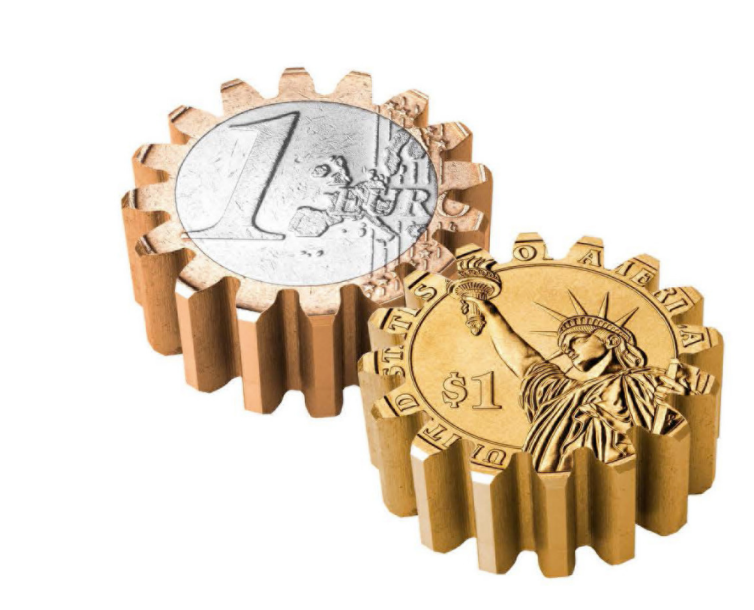
\includegraphics[width=0.9\linewidth]{Cover.png}
\end{column}

\end{columns}

% ----- Footer text (bottom-right corner) -----
\vspace*{2cm} % adjust if needed
\hfill{\large\textit{Prepared by Marcos Consuegra}}

\end{frame}


%-----------------------------------------------------------

\begin{frame}{What We Will Learn}
\small
\begin{itemize}
  \item What hyperinflation is (Cagan’s 50\% monthly threshold) and why it is largely a \textbf{modern, fiat-money} phenomenon.
  \item The empirical regularities: \textbf{money growth} and \textbf{inflation} move together; \textbf{real money balances collapse}; nominal interest rates surge.
  
  \item Three mechanisms behind high inflation/hyperinflation, and how each maps into equilibrium restrictions:
  \begin{itemize}
    \item explicit \textbf{deficit monetization} (fiscal dominance),
    \item \textbf{implicit backing} and fiscal capacity limits (\emph{unpleasant monetarist arithmetic}),
    \item \textbf{central-bank balance-sheet weakness} (insufficient backing / negative net worth).
  \end{itemize}
  
\end{itemize}
\end{frame}


% OUTLINE
\begin{frame}{Outline}
\tableofcontents
\end{frame}

% ===================== SECTION: INTRODUCTION =====================
\section{Introduction}

\begin{frame}{Hyperinflation}
\small

\textbf{Definition}
\begin{itemize}
    \item \textcite{cagan1956} defines \textbf{hyperinflation} as a monthly inflation rate exceeding \textbf{50\%}.
    \item This corresponds to an annualized inflation rate of approximately \textbf{12{,}875\%}.
\end{itemize}

\vspace{0.3cm}

\textbf{A Modern Rarity}
\begin{itemize}
    \item Pre-20th-century episodes were rare; one early case is associated with the French Revolution (1795--96) \parencite{capie1991}.
    \item Historically, hyperinflation was constrained by commodity-money regimes; modern cases (e.g.\ Zimbabwe, Venezuela) underscore the shift to fiat systems.
\end{itemize}
\end{frame}

% -----------------------------------------------------------

\begin{frame}{Historical Episodes}
\small
\textbf{Extreme Magnitude}
\begin{itemize}
    \item Hungary (1946): The most extreme case, monthly inflation reached $4.2 \times 10^{16}\%$.
    \item The price index rose from $1$ to $3.8 \times 10^{27}$ in months.
        \item By contrast, the price index during the French Revolution rose from $1$ to $18$.
\end{itemize}

\vspace{0.2cm}
\textbf{Frequency of High Inflation (1960--1996)}
\begin{itemize}
    \item While hyperinflation is rare, high-inflation episodes are frequent \parencite{fisher2002}:
\end{itemize}

\begin{table}[]
\footnotesize
\centering
\begin{tabular}{@{}lll@{}}
\toprule
\textbf{Annualized Inflation} & \textbf{Episodes} & \textbf{Countries} \\ \midrule
 $> 100\%$ & 45 & 25 \\
 $> 25\%$  & 212 & 92 \\ \bottomrule
\end{tabular}
\end{table}
\end{frame}

% -----------------------------------------------------------

\begin{frame}{Inconvertible Paper Currency}
\small

\textbf{The Removal of Convertibility}
\begin{itemize}
    \item Modern hyperinflations suggest a close connection to \textbf{inconvertible paper currency}.
    \item Currency is a central bank liability that can be expanded at discretion, without gold or silver convertibility.
    \item \textbf{Fiscal connection:} Inflation often reflects the expansion of \textbf{Treasury liabilities} that are effectively monetized by the central bank.
\end{itemize}

\vspace{0.3cm}

\textbf{Limitless Nominal Expansion}
\begin{quote}
    \textit{``Only inconvertible paper currencies can be expanded rapidly without limit to generate hyperinflation.''}
    --- \textcite{cagan1989hyper}
\end{quote}
\end{frame}


% -----------------------------------------------------------

\begin{frame}{Zimbabwe: A Contemporary Laboratory}
\centering
\vfill
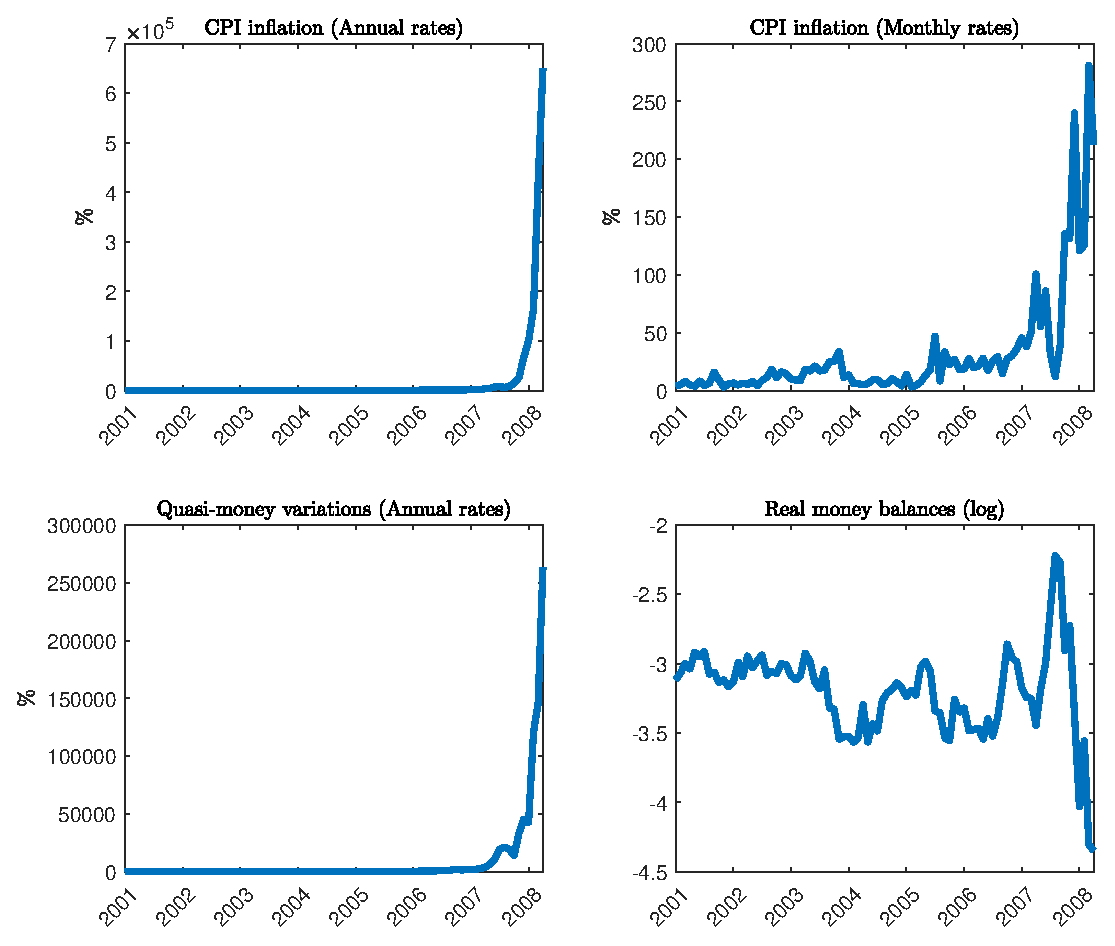
\includegraphics[width=0.68\textwidth,height=0.7\textheight,keepaspectratio]{Figures/Figure28.eps}

\vspace{0.2cm}
{\tiny inflation, money growth, and real balances in Zimbabwe (Jan 2001--Oct 2008).}\\
{\tiny \textit{Source: Central Statistical Office.}}
\vfill
\end{frame}

% -----------------------------------------------------------

\begin{frame}{Stylized Facts: Money, Prices, and Real Balances}
\small

\textbf{Hyperinflation as a Monetary Phenomenon}
\begin{itemize}
    \item Hyperinflations support the view that \textbf{inflation is a monetary phenomenon} (Friedman).
    \item \textbf{Empirical regularities:}
    \begin{itemize}
        \item Money growth and inflation are strongly correlated.
        \item Prices often outpace money growth, causing \textbf{real balances} to collapse.
    \end{itemize}
\end{itemize}

\vspace{0.2cm}

\textbf{\textcite{cagan1956} Money Demand}
\begin{itemize}
    \item Output movements can often be abstracted from, as they are \textbf{small} relative to the magnitude of price-level changes.
    \item \textbf{Implication:} Money demand is decreasing in \textbf{expected inflation}.
\end{itemize}
\end{frame}

% -----------------------------------------------------------

\begin{frame}{Monetary--Fiscal Coordination}
\small
\begin{itemize}
    \item Money growth is rarely a pure \enquote{monetary mistake}; it often reflects \textbf{coordinated fiscal and monetary actions} that sustain government spending.
    \item In wartime or post-war episodes, money creation may become the residual instrument for financing large expenditure shocks.
    \item Inflation can also be triggered by guarantees on Treasury debt or by insufficient \textbf{fiscal capacity} to back money with future taxes—\textbf{even without direct} deficit monetization.
    \item This fiscal--monetary link can also generate the \textbf{tight money paradox}: high interest rates intended to fight inflation may backfire if they worsen fiscal solvency (e.g., Brazil in the 1970s).
\end{itemize}
\end{frame}

% -----------------------------------------------------------

\begin{frame}{The Backing Requirement}
\small
\textbf{Asset Quality and the Monetary Anchor}
\begin{itemize}
    \item Institutional independence alone is not sufficient for price stability: a currency ultimately requires credible \textbf{fiscal or asset backing}.
    \item Absent Treasury support, the central bank’s portfolio (often claims on the banking sector) becomes the \textbf{sole anchor} for the currency.
    \item Large defaults on these assets can render the central bank insolvent, \textbf{forcing a debasement of the currency} to realign liabilities with diminished asset values.
    \item \textbf{Historical lesson:} The Bank of Amsterdam’s Dutch florin lost its global dominance in the 18th century after large losses—linked to loans to the Dutch East India Company—undermined the bank’s balance sheet \parencite{quinn2014}.
\end{itemize}
\end{frame}

% -----------------------------------------------------------

\begin{frame}{Empirical Evidence of Central Bank Strength}
\small
\textbf{Financial Strength and Stability}
\begin{itemize}
    \item \textcite{stella2008} documents a negative relationship between central bank net worth and inflation.
\end{itemize}

\vspace{0.2cm}

\begin{table}
\footnotesize
\centering
\begin{tabular}{@{}ll@{}}
\toprule
\textbf{Case Study} & \textbf{Outcome of Recapitalization} \\ \midrule
\textbf{Hungary (1997)}   & Inflation fell from 23\% to 11\%. \\
\textbf{Jamaica (1995)}   & Significant disinflation following financial restoration. \\ \bottomrule
\end{tabular}
\end{table}

\begin{itemize}
    \item \textbf{Chile’s exception:} Low inflation despite negative net worth, supported by \textbf{strong fiscal capacity} (very low net public debt).

\end{itemize}
\end{frame}

% -----------------------------------------------------------

\begin{frame}{Analytical Roadmap: Three Frameworks}
\small
The next sections analyze these dynamics through three complementary lenses:

\vspace{0.35cm}
\textbf{1. Explicit Deficit Monetization}
\begin{itemize}
    \item Money creation used to finance persistent Treasury deficits.
\end{itemize}

\vspace{0.2cm}
\textbf{2. Implicit Backing (\enquote{Unpleasant Arithmetic})}
\begin{itemize}
    \item Shared intertemporal resource constraints between the central bank and the Treasury generate inflationary equilibria even without direct monetization.
\end{itemize}

\vspace{0.2cm}
\textbf{3. Central Bank Solvency}
\begin{itemize}
    \item Inflation driven by balance-sheet losses, even under institutional separation.
\end{itemize}
\end{frame}

% -------------------- Outline of the Results --------------------
% -------------------- Outline of the Results --------------------
\section{Outline of the Results}

\begin{frame}{Outline of the Results}
\small
\begin{itemize}
    \item \textbf{Deficit Monetization}: Persistent fiscal deficits are financed through seigniorage, linking money growth, inflation, and the collapse of real balances.

    \vspace{0.3em}
    \item \textbf{Implicit Backing (\enquote{Unpleasant Arithmetic})}: Even without direct monetization, insufficient fiscal capacity and implicit guarantees generate inflationary equilibria and can deliver \textbf{multiple steady states}.

    \vspace{0.3em}
    \item \textbf{Central Bank Solvency}: Central bank net worth matters for monetary control; insolvency (under non-negative remittances) can force inflation through the need to generate seigniorage.
\end{itemize}
\end{frame}


% ===================== SECTION: DEFICIT FINANCING =====================
\section{Deficit Financing and Inflation}

\begin{frame}{Hyperinflation: Deficit Monetization}
\small
\textbf{The Seigniorage Problem}
\begin{itemize}
    \item Treasuries typically finance deficits through taxation or market borrowing.
    \item When access to markets is restricted and tax hikes are unviable, policymakers often resort to central bank \textbf{seigniorage}—issuing money to cover deficits.
    \item Persistent reliance on the printing press is a primary driver of hyperinflationary episodes.
\end{itemize}

\vspace{0.3cm}

\textbf{Analytical Assumptions}
\begin{itemize}
    \item In what follows, real output is assumed to be constant, as variations in the real sector are negligible compared with the extreme magnitude of price‑level movements.
    \item The following framework restates the equilibrium conditions from Chapter 2, where the central bank issues both reserves and cash.
\end{itemize}
\end{frame}

% -----------------------------------------------------------
\begin{frame}{Equilibrium Conditions: The Fisher Equation}
\small
The first fundamental relation linking the nominal interest rate to inflation is the \textbf{Fisher equation}:
\begin{equation}
1 + i_{t} = \frac{1}{\beta}\,\frac{P_{t+1}}{P_{t}}
\label{Fisher-I}
\end{equation}

\textbf{Interpretation}
\begin{itemize}
    \item $i_t$: the nominal interest rate.
    \item $1/\beta$: the (constant) real interest rate.
    \item $P_t$: the price level.
\end{itemize}
\end{frame}

\begin{frame}{Money Market Equilibrium}
\small
The money‑market equilibrium links \textbf{real money balances} to the nominal interest rate:
\begin{equation}
\frac{M_{t}}{P_{t}} = L(i_t)
\label{MD-I}
\end{equation}

\textbf{Interpretation}
\begin{itemize}
    \item $M_t$: nominal money holdings.
    \item $L(\cdot)$: a decreasing function of the nominal interest rate $i_t$.
    \item Demand for real balances falls as the opportunity cost of holding money ($i_t$) rises.
\end{itemize}
\end{frame}

\begin{frame}{The Cagan Relationship}
\small
Combining the Fisher equation \eqref{Fisher-I} with the money‑market equilibrium \eqref{MD-I} yields the Cagan relation:
\[
\frac{M_t}{P_t} = \tilde{L}\!\bigl(P_t/P_{t+1}\bigr),
\]
where \(\tilde{L}\) is the money‑demand function \(L(i_t)\) re‑expressed as a decreasing function of the expected gross inflation \(P_t/P_{t+1}\).

\vspace{0.2cm}

\textbf{Interpretation}
\begin{itemize}
    \item Real money balances are a decreasing function of expected inflation: higher expected inflation reduces money demand.
    \item \(\tilde{L}\) captures the same behavioural relationship as \(L(i_t)\), but in terms of inflation expectations rather than interest rates.
\end{itemize}
\end{frame}


% -----------------------------------------------------------
\begin{frame}{Treasury Flow Budget Constraint}
\small
The Treasury’s flow budget constraint is:

\begin{equation}
\frac{B_{t}^{F}}{1+i_{t}}=B_{t-1}^{F}+\mathcal{D}_{t}-T_{t}^{C}. \label{FlowT}
\end{equation}

\vspace{0.4cm}
\textbf{Interpretation}
\begin{itemize}
    \item $B_{t}^{F}$: Total Treasury debt issued at time $t$.
    \item $\mathcal{D}_{t}$: Primary deficit ($\mathcal{D}_{t} > 0$) or surplus ($\mathcal{D}_{t} < 0$).
    \item $T_{t}^{C}$: Central Bank remittances (transfers) to the Treasury.
\end{itemize}
\end{frame}

% -----------------------------------------------------------
\begin{frame}{Central Bank Flow Budget Constraint}
\small
The central bank manages its assets and liabilities while determining the level of remittances:

\begin{equation}
\frac{B_t^{C}-X_t}{1+i_t}\,-\,M_t = B_{t-1}^{C} - X_{t-1} - M_{t-1} - T_t^{C}.
\label{FlowBCI}
\end{equation}

\vspace{0.4cm}
\textbf{Interpretation}
\begin{itemize}
    \item \(B_t^{C}\): central‑bank holdings of short‑term assets.
    \item \(X_t\): central‑bank reserves (liabilities).
    \item \(M_t\): central‑bank money, i.e., cash and/or banknotes.
    \item \(T_t^C\): remittances (or transfers) paid by the central bank to the treasury.
\end{itemize}
\end{frame}
% -----------------------------------------------------------
\begin{frame}{The Intertemporal Resource Constraint}
\small
The model is closed by consolidating the Treasury and Central Bank constraints into a single public sector resource constraint, using $B_t^F = B_t^C +B_t$:

\begin{equation}
\sum_{t=t_{0}}^{\infty }\beta ^{t-t_{0}}\left( \frac{i_{t}}{1+i_{t}}\frac{M_{t}}{P_{t}}-\frac{\mathcal{D}_{t}}{P_{t}}\right) = \frac{B_{t_{0}-1} + X_{t_{0}-1} + M_{t_{0}-1}}{P_{t_{0}}} \label{IBC-I}
\end{equation}
\vspace{0.4em}
\begin{itemize}
    \item Following Chapter 2, this is the mirror image of the consumers' intertemporal budget constraint, derived from goods and asset market-clearing conditions.
    \item \textbf{Note}: It is not a solvency condition but an intertemporal resource constraint that holds in equilibrium.
\end{itemize}
\end{frame}
% -----------------------------------------------------------
% -----------------------------------------------------------
% -----------------------------------------------------------
\begin{frame}{Deficit Specification}
\small
We set an exogenous path for the \textbf{real} fiscal deficit $\{\mathsf{d}_{t}\}_{t=t_{0}}^{\infty}$, where $\mathsf{d}_{t} \equiv \mathcal{D}_{t}/P_{t}$. 
\vspace{0.3em}

The path of this deficit during hyperinflation is determined by two competing effects:

\begin{itemize}
    \item \textbf{Keynes--Tanzi Effect (Deficit Expansion)}
    \begin{itemize}
        \item Tax collection lags erode the real value of fiscal revenues. For a given path of real expenditures, this leads to an \textbf{increase} in the real deficit.
        \item This can create a self-reinforcing spiral where higher inflation necessitates even more seigniorage.
    \end{itemize}
    
    \vspace{0.2cm}
    \item \textbf{Patinkin Effect (Deficit Contraction)}
    \begin{itemize}
        \item If spending is fixed in nominal terms, its real value falls as prices rise. If taxes are indexed, the real deficit may actually \textbf{fall}.
    \end{itemize}
\end{itemize}
\end{frame}


% -----------------------------------------------------------
\begin{frame}{Seigniorage}
\small
\begin{itemize}
    \item \textbf{Bond Market Assumption}: All treasury debt is held by the central bank ($B_{t}^{F}=B_{t}^{C}$ and $B_{t}=0$).
    \item \textbf{Financing Identity}: Each period’s deficit and maturing debt are financed by new debt held by the central bank and received remittances:
    \begin{equation*}
    P_{t}\mathsf{d}_{t}+B_{t-1}^{C}=\frac{B_{t}^{C}}{1+i_{t}}+T_{t}^{C}.
    \end{equation*}
    \item Substituting the central bank's flow budget constraint \eqref{FlowBCI} and assuming zero reserves, i.e. $X_{t}=0$, we obtain the fundamental deficit-seigniorage relation:
    \begin{equation}
    \mathsf{d}_{t}=\frac{M_{t}-M_{t-1}}{P_{t}}. \label{Deficit}
    \end{equation}
    \item \textbf{Result}: The real deficit is funded entirely by money creation.
\end{itemize}
\end{frame}

% -----------------------------------------------------------
\begin{frame}{Monetary Policy and Cagan Demand}
\small
\begin{itemize}
    \item \textbf{Monetary rule:} The money supply grows at a constant rate,
    \(M_{t}=(1+\vartheta)\,M_{t-1}\). Financing a persistent deficit implies \(\vartheta>0\).

    \item \textbf{Cagan demand specification:} Following \textcite{cagan1956}, real money balances depend on expected gross inflation
    \(\Pi_{t+1}\equiv P_{t+1}/P_{t}\) through the inverse-inflation formulation:
    \begin{equation}
    \frac{M_{t}}{P_{t}}
    = \tilde{L}\!\Bigl(\tfrac{1}{\Pi_{t+1}}\Bigr)
    = \bigl(\Pi_{t+1}\bigr)^{-\lambda_{\pi}},
    \label{Cagan2}
    \end{equation}
    where \(\lambda_{\pi}>0\). This is a particular functional-form specification for \(\tilde{L}\).
\end{itemize}
\end{frame}



\begin{frame}{Dynamics of Real Money Balances}
\small

\begin{itemize}
    \item Define \textbf{real money balances} as
    \[
        m_t \equiv \frac{M_t}{P_t}.
    \]
    \item Substituting the money growth rule \(M_t=(1+\vartheta)M_{t-1}\) into the Cagan demand equation \eqref{Cagan2} yields:
\end{itemize}

\vspace{0.2cm}
\textbf{Law of motion}
\begin{equation*}
m_{t}=\left( \frac{m_{t}}{m_{t+1}}(1+\vartheta )\right) ^{-\lambda _{\pi }} .
\end{equation*}

\begin{itemize}
    \item Rearranging gives the non-linear difference equation:
    \begin{equation}
    m_{t+1}=m_{t}^{1+\frac{1}{\lambda _{\pi }}}(1+\vartheta ).
    \label{eq: RMB}
    \end{equation}

    \item \textbf{Stationary solution:} point \(E\), where \(m=(1+\vartheta)^{-\lambda_{\pi}}\). In this state, prices and money grow at the same rate (\(\Pi=1+\vartheta\)).
\end{itemize}

\end{frame}

% -----------------------------------------------------------
\begin{frame}{Phase Diagram}
\centering
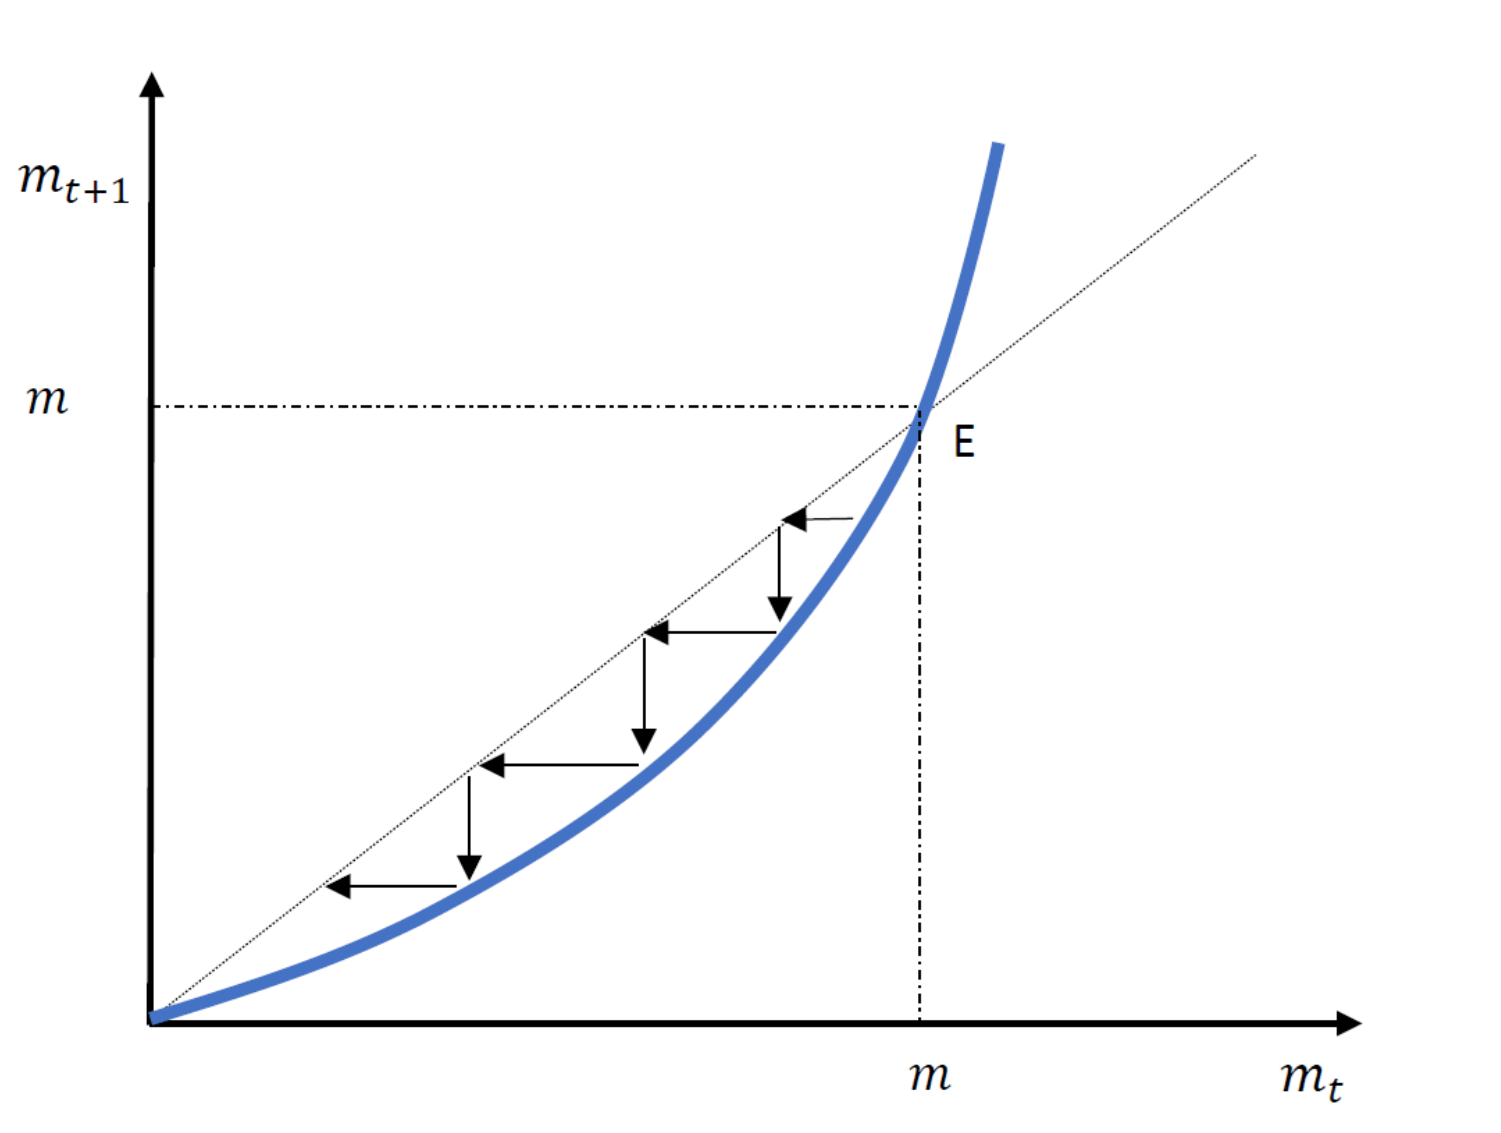
\includegraphics[width=0.55\linewidth]{Figures/Figure29.PNG}
\par
\vspace{0.2cm}
\textit{\tiny Dynamics of the difference equation (\ref{eq: RMB}). Paths to the left of the stationary point $E$ characterize the hyperinflationary "flight from currency." In these trajectories, rising interest rates increase the opportunity cost of holding cash, forcing inflation to accelerate beyond the rate of money growth.}
\end{frame}

% -----------------------------------------------------------
\begin{frame}{Equilibrium Seigniorage and Real Balances}
\small
\begin{itemize}
    \item Following \textcite{bruno1990}, assume the \textbf{real deficit is constant}:
    \[
      \mathsf{d}_t = \mathsf{d}.
    \]
    \item Using \(M_{t-1}=(1+\vartheta)^{-1}M_t\) in the deficit equation \eqref{Deficit}, we obtain
    \[
    \mathsf{d}
    =\frac{M_t-M_{t-1}}{P_t}
    =\left(1-\frac{1}{1+\vartheta}\right)\frac{M_t}{P_t}
    =\frac{\vartheta}{1+\vartheta}\,m_t,
    \qquad
    m_t \equiv \frac{M_t}{P_t}.
    \]
    \item Since \(\mathsf{d}\) and \(\vartheta\) are constant, equilibrium requires \textbf{constant real balances}: \(m_t = m\).
    \item \textbf{Note:} With a constant real deficit and constant money growth, this framework cannot generate collapsing real balances; such dynamics require time-varying paths (e.g.\ changing \(\mathsf{d}_t\) or \(\vartheta_t\)). 
\end{itemize}
\end{frame}


% -----------------------------------------------------------
\begin{frame}{The Seigniorage Laffer Curve}
\small
\begin{itemize}
    \item Combining the steady state \(m=(1+\vartheta)^{-\lambda_\pi}\) with the seigniorage condition implies
    \begin{equation}
        \mathsf{d} = \vartheta (1+\vartheta)^{-\lambda_\pi - 1}.
        \label{dv}
    \end{equation}
    \item Seigniorage is maximized at \(\vartheta^{*} = 1/\lambda_\pi\).
    \item Using Cagan’s (1956) estimate \(\lambda_\pi \approx 4.68\), the revenue-maximizing money growth rate is approximately \textbf{20\% per month}.
    \item \textbf{Equilibrium:}
    \begin{enumerate}
        \item If \(\mathsf{d} > \mathsf{d}_{\max}\), no equilibrium exists.
        \item If \(\mathsf{d} < \mathsf{d}_{\max}\), two growth rates \((\vartheta_L,\vartheta_H)\) can finance the deficit.
    \end{enumerate}
    \item \textbf{Note:} \(\vartheta\) is a policy choice; conditional on the central bank selecting \(\vartheta\), the equilibrium path is pinned down.
\end{itemize}
\end{frame}

% -----------------------------------------------------------
\begin{frame}{Missing Time Variation}
\small
\begin{itemize}
    \item With a constant real deficit and constant money growth, equilibrium implies constant real balances, so the model cannot generate a \enquote{flight from currency.}
    \vspace{0.4em}
    \item To match historical hyperinflations, the model requires time variation in:
    \begin{itemize}
        \item \textbf{Fiscal policy:} time-varying deficits \(\mathsf{d}_t\) (e.g., tax-collection lags).
        \item \textbf{Monetary policy:} time-varying money growth rates \(\vartheta_t\).
    \end{itemize}
\vspace{0.4em}
\item Despite these limits, the framework isolates the tight link between deficit finance through seigniorage, money growth, and inflation.
\end{itemize}
\end{frame}

% -----------------------------------------------------------
\begin{frame}{Causality}
\small
The model provides a twofold answer to the causality of hyperinflation:
\vspace{0.2cm}
\begin{itemize}
    \item \textbf{Monetary mechanism:} Inflation is proximately driven by money growth, because seigniorage is the operational instrument used to finance deficits.
    \item \textbf{Fiscal root:} The underlying cause is \textbf{unsustainable fiscal policy}—persistent deficits without a credible path of adjustment.
    \item \textbf{Independence counterfactual:} A truly independent central bank could refuse monetization, forcing the Treasury into a binary choice:
    \begin{enumerate}
        \item \textbf{Fiscal adjustment:} restore solvency through spending cuts or tax increases.
        \item \textbf{Sovereign default:} if adjustment is not feasible, default on obligations.
    \end{enumerate}
    \item \textbf{Conclusion:} Hyperinflation reflects a breakdown of \textbf{fiscal–monetary coordination}.
\end{itemize}
\end{frame}


% -----------------------------------------------------------
\begin{frame}{Nominal Deficit}
\small
\textbf{Nominal Deficit Specification}
\begin{itemize}
    \item We now consider a regime where the Treasury's deficit is fixed in nominal terms, $\{\mathcal{D}_t\}_{t=t_0}^{\infty}$.
    \item The nominal deficit and maturing debt are financed via Central Bank remittances and bond issuance:
    \begin{equation*}
    \mathcal{D}_{t}+B_{t-1}^{C}=\frac{B_{t}^{C}}{1+i_{t}}+T_{t}^{C}.
    \end{equation*}
    \item  With $X_t = 0$, the time-variation of the money supply is determined by the nominal fiscal requirement:
    \begin{equation*}
    M_{t}=\mathcal{D}_{t}+M_{t-1}.
    \end{equation*}
    \item  Assuming a constant ratio $\mathcal{D}_t/M_{t-1} = \vartheta$, money growth becomes $M_t = (1+\vartheta)M_{t-1}$.
    \item \textbf{Result}: Unlike the real-deficit case, $\vartheta$ is uniquely dictated by fiscal policy rather than being a monetary-policy choice.
\end{itemize}
\end{frame}

% -----------------------------------------------------------
\begin{frame}{Dynamics and Multiplicity of Equilibria}
\small
\begin{itemize}
    \item Combining the money-supply rule with the money market equilibrium \eqref{Cagan2} using \eqref{eq: RMB} yields a non-linear difference equation in real balances:
    \[
        m_{t+1}=m_{t}^{1+\frac{1}{\lambda _{\pi }}}(1+\vartheta ). \label{eq: RMB_Nom}
    \]
    \item \textbf{Existence}: Unlike real-deficit regimes, a solution exists for any $\vartheta > 0$. 
    \item \textbf{The Multiplicity Problem}: One $\vartheta$ allows three distinct types of paths:
    \begin{enumerate}
        \item \textbf{Stationary}: $m_t$ remains constant at $m = (1+\vartheta)^{-\lambda_{\pi}}$.
        \item \textbf{Hyperinflationary}: $m_t \to 0$ as inflation outpaces money growth.
        \item \textbf{Deflationary Bubbles}: $m_t \to \infty$ as prices fall. This solution is ruled out by the transversality condition.
    \end{enumerate}
\end{itemize}
\end{frame}


% -----------------------------------------------------------
\begin{frame}{The Hyperinflationary Equilibrium}
\small
Consistent with empirical evidence, the model admits non-stationary equilibria where real money balances fall over time as inflation consistently outpaces money growth ($\pi_t > \vartheta$).

\vspace{0.2cm}
\begin{itemize}
    \item \textbf{Rising Opportunity Cost}: Interest rates keep increasing, making it more costly to hold real money balances and reinforcing the downward trajectory of $m_t$.
    
    \item \textbf{Endogenous Real Adjustment}: Unlike the previous example, the real deficit $\mathsf{d}_t$ is not a choice, but follows the path of real money balances:
    \begin{equation*}
    \mathsf{d}_{t}=\frac{\vartheta }{1+\vartheta }m_{t}.
    \end{equation*}
    
    \item \textbf{The Result}: Even as the government meets its \textbf{nominal} growth target $\vartheta$, the \textbf{real} value of its deficit financing vanishes. Inflation acts as a tax that eventually destroys its own tax base.
\end{itemize}
\end{frame}
% -----------------------------------------------------------

% -----------------------------------------------------------
\begin{frame}{Hyperinflations with Interest-Rate Policies}
\small
Hyperinflation is not peculiar to money-growth rules: it can also arise under interest-rate policy when the central bank sets the interest rate on reserves.

\begin{itemize}
    \item Whether policy is implemented through money supply or interest rates, the key feature is that \textbf{fiscal policy ultimately commands monetary policy}.
    
    \item Define central bank net worth:
    \[
      N_t^{C} \;\equiv\; \frac{B_t^{C}-X_t}{1+i_t} \;-\; M_t.
    \]
    
    \item The flow budget constraint \eqref{FlowBCI} can be rewritten as the law of motion for net worth:
    \[
      N_t^{C} \;=\; N_{t-1}^{C} + \Psi_t^{C} - T_t^{C},
    \]
    where profits satisfy
    \[
      \Psi_t^{C} = i_{t-1}\bigl(N_{t-1}^{C}+M_{t-1}\bigr).
    \]
\end{itemize}
\end{frame}


% -----------------------------------------------------------
\begin{frame}{Policy Assumptions and Remittances}
\small
To isolate the mechanics of interest-rate policies, we assume a regime of fiscal subordination:

\begin{itemize}
    \item Initial net worth is zero \((N_{t_{0}-1}^{C}=0)\), and all profits are rebated to the Treasury \((T_{t}^{C}=\Psi _{t}^{C})\), implying \(N_t^C = 0\) for all \(t\).
    \item These assumptions require assets and liabilities to match exactly in every period:
    \begin{equation}
    \frac{B_{t}^{C}}{1+i_{t}}=\frac{X_{t}}{1+i_{t}}+M_{t}. \label{BSCentral Bank}
    \end{equation}
    \item Given \(N_{t-1}^C = 0\), the profit definition implies that remittances reduce to the interest earned on the monetary base:
    \begin{equation*}
    T_{t}^{C}=i_{t-1}M_{t-1}.
    \end{equation*}
\end{itemize}
\end{frame}


% -----------------------------------------------------------
\begin{frame}{Deficit Financing via High-Powered Money}
\small
\begin{itemize}
    \item Assume a constant real deficit \(\mathsf{d}\) is financed exclusively through central bank remittances and central bank–held debt:
    \[
    P_{t}\mathsf{d}+B_{t-1}^{C}=\frac{B_{t}^{C}}{1+i_{t}}+T_{t}^{C}.
    \]
    \item Substituting the balance sheet condition \eqref{BSCentral Bank} and the remittance rule yields
    \begin{equation}
    P_{t}\mathsf{d}+X_{t-1}+M_{t-1}=\frac{X_{t}}{1+i_{t}}+M_{t}.
    \label{Deficit-X}
    \end{equation}
    \item Thus, the fiscal deficit is ultimately financed by an expansion in central bank liabilities—i.e.\ by \textbf{high-powered money}.
\end{itemize}
\end{frame}


% -----------------------------------------------------------
% -----------------------------------------------------------
\begin{frame}{The Intertemporal Resource Constraint}
\small
\begin{itemize}
    \item Iterating the consolidated flow condition \eqref{Deficit-X} forward and imposing the intertemporal constraint \eqref{IBC-I} yields:
\end{itemize}

\vspace{0.2cm}
\textbf{Intertemporal resource constraint}
\begin{equation}
\frac{b_{t_{0}-1}^{g}}{\Pi _{t_{0}}}+\mathsf{d}
=(1-\beta)\sum_{t=t_{0}}^{\infty }\beta ^{t-t_{0}}
\left( \frac{i_{t}}{1+i_{t}}\frac{M_{t}}{P_{t}}\right),
\label{Key}
\end{equation}
\hspace{0.65cm} where outstanding real liabilities are
\(b_{t_{0}-1}^{g}\equiv (1-\beta)(X_{t_{0}-1}+M_{t_{0}-1})/P_{t_{0}-1}\).

\begin{itemize}
    \item This condition jointly restricts the initial price jump \(\Pi_{t_0}\) and the entire future path of nominal interest rates \(\{i_t\}_{t\ge t_0}\).
\end{itemize}
\end{frame}

% -----------------------------------------------------------
\begin{frame}{Seigniorage Requirements}
\small
\begin{itemize}
    \item Suppose \(i_t=i\) for all \(t\ge t_0\). By the Fisher equation \eqref{Fisher-I}, inflation is constant at
    \[
        \Pi=\beta(1+i).
    \]
    \item Combining \eqref{Key} with Cagan money demand \eqref{Cagan2} implies the steady-state restriction
    \begin{equation}
    \frac{b_{t_{0}-1}^{g}}{\Pi _{t_{0}}}
    =\left( \frac{\Pi -\beta }{\Pi }\right)\Pi ^{-\lambda _{\pi }}-\mathsf{d}.
    \label{Key2}
    \end{equation}
    \item Since \(b_{t_0-1}^g>0\), the right-hand side must be strictly positive for an equilibrium to exist.
    \item Hence, seigniorage revenues must be sufficiently large to cover the real fiscal deficit \(\mathsf{d}\).
\end{itemize}
\end{frame}

% -----------------------------------------------------------
\begin{frame}{Seigniorage Properties}
\small
\begin{itemize}
    \item The properties of the seigniorage term in \eqref{Key2} define the limits of monetization:
\end{itemize}

\vspace{0.2cm}

\begin{itemize}
    \item Revenue follows a Laffer-curve shape: it is zero at $\Pi=\beta$ and as $\Pi\to\infty$.
    \vspace{0.25em}
    \item Seigniorage is maximized at
    \[
        \Pi=\beta\left(1+\lambda_{\pi}^{-1}\right).
    \]
    \vspace{0.25em}
    \item Using Cagan’s estimates, the maximum occurs at approximately \textbf{20\% monthly inflation}.
    \vspace{0.25em}
    \item Deficits above this peak are not consistent with an equilibrium under a constant interest-rate policy.
\end{itemize}
\end{frame}


% -----------------------------------------------------------
\begin{frame}{Initial Inflation and Policy Selection}
\small

\begin{itemize}
    \item Using (\ref{Key2}), the central bank must set an interest rate $i$ that generates enough seigniorage to cover $\mathsf{d}$.
    \item Once policy is set, inflation at time $t_0$ ($\Pi_{t_0}$) adjusts to clear the public sector's intertemporal budget.
    \item There is an inverse relationship: higher future seigniorage extraction allows for a lower initial inflation jump.
    \item Dual solutions for the nominal interest rate may exist; this represents two distinct policy paths consistent with the same fiscal requirement.
\end{itemize}
\end{frame}

% -----------------------------------------------------------
\begin{frame}{Irrelevance of the Monetary Instrument}
\small
The analysis shows that the choice of monetary instrument (money versus interest rate) does not materially change the outcome:

\begin{itemize}
    \item The critical ingredient is the \textbf{subordination of monetary policy to fiscal needs}.
    \item Across specifications, inflation is driven by the same force: reliance on \textbf{seigniorage} to finance persistent deficits.
    \item This logic is consistent with hyperinflation episodes, which feature collapsing real balances and soaring nominal interest rates.
\end{itemize}
\end{frame}


% ----------------------------------------------------------

% -----------------------------------------------------------
\section{Some Unpleasant Monetarist Arithmetic}

\begin{frame}{Hyperinflation without Direct Monetary Financing}
\small
The central bank’s control of inflation can hinge on subtle fiscal–monetary coordination:

\begin{itemize}
    \item Coordination may be implicit: Treasury debt is effectively backed so that it acquires the same \enquote{default-free} status as central bank's liabilities.
    \item Under such a guarantee, the binding constraint on Treasury borrowing is not repayment, but its eventual inflationary consequences.
    \item Backing can be explicit (e.g., purchases financed by reserves) or implicit; inflation emerges when fiscal capacity is insufficient to support the guarantee.
    \item Once an implicit guarantee is in place, the central bank loses the ability to conduct fully independent policy—even in the absence of direct deficit monetization.
    \item Government liabilities are then perceived as monetary backstops, subordinating the nominal anchor to fiscal solvency.
\end{itemize}
\end{frame}


\begin{frame}{The Intertemporal Constraint with Treasury Debt}
\small
\begin{itemize}
    \item Assume a constant real deficit \(\mathsf{d}\). The intertemporal equilibrium condition \eqref{IBC-I} implies a fundamental link between seigniorage and total public liabilities:
\end{itemize}

\vspace{0.2cm}
\textbf{Consolidated resource constraint}
\begin{equation}
(1-\beta )\sum_{t=t_{0}}^{\infty }\beta ^{t-t_{0}}
\left( \frac{M_{t}-M_{t-1}}{P_{t}}\right)
-\mathsf{d}
=\frac{b_{t_{0}-1}^{G}}{\Pi _{t_{0}}}.
\label{Key-Hyper}
\end{equation}

\begin{itemize}
    \item Total real liabilities are defined as
    \[
      b_{t_{0}-1}^{G}\equiv (1-\beta )\frac{B_{t_{0}-1}+X_{t_{0}-1}}{P_{t_{0}-1}},
    \]
    capturing net private-sector holdings of Treasury debt and central bank reserves.
    \item We restrict attention to non-deflationary equilibria in which the discounted value of future real money holdings vanishes:
    \[
      \lim_{t\to \infty} \beta^{t-t_{0}}\frac{M_{t-1}}{P_{t}}=0.
    \]
\end{itemize}
\end{frame}




% -----------------------------------------------------------
% -----------------------------------------------------------
\begin{frame}{Policy Restrictions and Equilibrium}
\small
\begin{itemize}
    \item The intertemporal condition \eqref{Key-Hyper} is an \textbf{equilibrium restriction}, not a solvency constraint, because Treasury liabilities are implicitly backed by the central bank.
    \item Therefore, even without direct deficit monetization, \eqref{Key-Hyper} must hold in equilibrium.
    \item The Treasury’s choice of the real deficit \(\mathsf{d}\) effectively constrains the feasible path of monetary policy.
    \item \textbf{Interpretation:} Inflation is not merely a monetary phenomenon; it is the adjustment mechanism that aligns the real value of public liabilities with the present value of future fiscal resources.
\end{itemize}
\end{frame}


% -----------------------------------------------------------
\begin{frame}{Restriction on the Path of Money Supply}
\small
\begin{itemize}
    \item The equilibrium condition \eqref{Key-Hyper} implies that monetary policy cannot remain fully independent indefinitely when public liabilities and deficits are positive.
    \item If \(b_{t_{0}-1}^{G}>0\) and \(\mathsf{d}>0\), there is no equilibrium in which the money supply remains constant for all \(t\).
    \item Eventually, the public sector budget forces the monetary authority to expand the money supply.
    \item Under constant money growth, \(M_{t}=(1+\vartheta)M_{t-1}\), the constraint becomes
    \begin{equation}
    \frac{\vartheta (1-\beta )}{(1+\vartheta )}\left( \sum_{t=t_{0}}^{\infty}\beta ^{t-t_{0}}m_{t}\right)
    =\mathsf{d}+\frac{b_{t_{0}-1}^{G}}{\Pi _{t_{0}}}.
    \label{Key-Hyper2}
    \end{equation}
\end{itemize}
\end{frame}

% -----------------------------------------------------------
\begin{frame}{Dynamics of Real Money Balances}
\small
\begin{itemize}
    \item Real money-balance dynamics are governed jointly by money growth and Cagan money demand.
    \item From Cagan demand \eqref{Cagan2}, the law of motion for real balances satisfies
    \begin{equation}
    m_{t+1}=m_{t}^{1+\frac{1}{\lambda _{\pi }}}(1+\vartheta).
    \label{Cagan3}
    \end{equation}
    \item The system admits a stationary solution \(m_t=m=(1+\vartheta)^{-\lambda_\pi}\).
    \item Crucially, it also admits non-stationary paths with declining real balances (\(m_t<m\)), capturing a \enquote{flight from currency}.
\end{itemize}
\end{frame}

% -----------------------------------------------------------
\begin{frame}{Stationary Equilibrium Conditions}
\small
\begin{itemize}
    \item Substituting the stationary solution into \eqref{Key-Hyper2} yields the stationary restriction linking fiscal and monetary variables:
    \begin{equation}
    \frac{b_{t_{0}-1}^{G}}{\Pi _{t_{0}}}+\mathsf{d}
    =\vartheta (1+\vartheta)^{-(\lambda _{\pi }+1)}.
    \label{Eq:I1}
    \end{equation}

    \item Using the identity \(m_{t_0}=m_{t_0-1}(1+\vartheta)/\Pi_{t_0}\) together with the stationary condition
    \(m_{t_0}=(1+\vartheta)^{-\lambda_\pi}\), we obtain the initial inflation jump:
    \[
        \Pi_{t_0}=(1+\vartheta)^{\lambda_\pi+1}\,m_{t_0-1}.
    \]

    \item \textbf{Key insight:} Unlike explicit deficit monetization, the stock of public liabilities \(b^{G}\) directly constrains the feasible paths for inflation and the monetary stance through the intertemporal equilibrium condition.
\end{itemize}
\end{frame}

% -----------------------------------------------------------
\begin{frame}{Solving for the Money Growth Rate}
\small
\begin{itemize}
    \item Combining the initial inflation jump with the resource constraint yields the key equation pinning down the money growth rate \(\vartheta\):
    \begin{equation}
    \vartheta
    =\mathsf{d}(1+\vartheta )^{(\lambda _{\pi }+1)}
    +\frac{b_{t_{0}-1}^{G}}{m_{t_{0}-1}}.
    \label{Eq: Vu}
    \end{equation}

    \item For sufficiently low values of \(\mathsf{d}\) and \(b_{t_0-1}^{G}\), this equation admits two solutions, \(\vartheta_{L}\) and \(\vartheta_{H}\).
    \item These correspond to two distinct stationary inflation rates that are consistent with the same fiscal requirement.
\end{itemize}
\end{frame}

% -----------------------------------------------------------
\begin{frame}{Fiscal Policy Dominance}
\small
\begin{itemize}
    \item \textbf{The fiscal limit:} Equilibrium existence is bounded by the arithmetic of \eqref{Eq: Vu}. If the deficit \(\mathsf{d}\) or initial debt \(b_{t_0-1}^{G}\) is too large, the relevant mapping fails to admit a solution and no equilibrium exists.

    \item \textbf{Fiscal dominance:} The Treasury effectively leads. Even without direct monetization, the central bank is forced into a monetary accommodation to satisfy \eqref{Key-Hyper} under the implicit backstop.

    \item \textbf{Two stationary solutions:} When debt and deficits are sustainable, two stationary outcomes exist: \(\vartheta_L\) (low inflation) and \(\vartheta_H\) (high inflation). The selection between them is ultimately a monetary policy choice: uniqueness of equilibrium.
\end{itemize}
\end{frame}

\begin{frame}{The Role of Outstanding Liabilities}
\small
\begin{itemize}
    \item The transition to implicit backing highlights that outstanding liabilities can drive inflation as much as current fiscal flows.
    \item Even a fiscal surplus (\(\mathsf{d}<0\)) can be associated with positive inflation if the inherited liability stock \(b_{t_{0}-1}^{G}\) is sufficiently large.
    \item Inflation arises whenever fiscal capacity is insufficient to back the outstanding stock of liabilities:
    \[
        -\mathsf{d} < \frac{b_{t_{0}-1}^{G}}{m_{t_{0}-1}}.
    \]
    \item A zero money-growth equilibrium can exist only if the surplus exactly offsets the inherited liability stock.
    \item This \enquote{unpleasant arithmetic} shows that the price level and inflation are ultimately anchored by intertemporal resource constraints on the consolidated public-sector balance sheet.
\end{itemize}
\end{frame}


% -----------------------------------------------------------
\begin{frame}{Hyperinflation and the Flight from Money}
\small


\begin{itemize}
\item Non-stationary equilibria allow for accelerating inflation even with constant policy parameters.
    \item Beyond stationary solutions, hyperinflationary paths exist where real money balances $m_t$ fall continuously.
    \item These paths are triggered by an initial price jump $\Pi_{t_0}$ that exceeds the stationary level to satisfy \eqref{Key-Hyper2}.
    \item This represents a rational anticipation of future monetization, leading to a flight from currency.
    \item Once the central bank’s guarantee is understood, monetary policy cannot contain inflation independently of fiscal capacity.
\end{itemize}
\end{frame}



% -----------------------------------------------------------
\begin{frame}{Sargent-Wallace Experiment: Resisting Inflation}
\small

\begin{itemize}
\item We analyze a scenario where the central bank attempts to resist inflation by tightening money today, only to succumb later (\cite{sargent1981}).
    \item \textbf{Tight Money Phase}: $M_t = M_{t_0-1}$ for $t_0 \leq t \leq T$.
    \item \textbf{Monetization Phase}: $M_{t+1} = (1+\vartheta^{\prime})M_t$ for $t \geq T$.
    \item For $t \geq T$, real balances are stationary ($m_T = (1+\vartheta^{\prime})^{-\lambda_\pi}$).
\end{itemize}
\end{frame}

% -----------------------------------------------------------
\begin{frame}{Dynamics of the "Tight Money" Phase}
\small
Even while money supply is held constant ($t < T$), the price level continues to rise:

\begin{itemize}
    \item During the tight money phase ($\vartheta = 0$), real balances follow:
    \begin{equation}
    m_{t+1}=m_{t}^{1+\frac{1}{\lambda _{\pi }}}. \label{eq: Rm1}
    \end{equation}
    \item Because $m_T<1$, real balances must fall over time toward that steady state.
    \item Consequently, inflation is positive during the "tight" phase as the public anticipates the eventual monetary surrender.
\end{itemize}
\end{frame}

% -----------------------------------------------------------
\begin{frame}{The Unpleasant Arithmetic of Surrender}
\small


\begin{itemize}
\item Integrating the transition path into the intertemporal constraint \eqref{Key-Hyper} reveals the fundamental trade-off of delayed action:
    \begin{equation}
    \beta ^{T+1-t_{0}}\frac{\vartheta ^{\prime }(1+\vartheta ^{\prime })^{-(\lambda _{\pi }+1)}}{1-\beta }-\mathsf{d}=\frac{b_{t_{0}-1}^{G}}{\Pi _{t_{0}}^{^{\prime }}}. \label{EqI2}
    \end{equation}
    \item Comparing this to immediate monetization shows that tight money today forces either higher future seigniorage ($\vartheta' > \vartheta$) or a sharper current inflation jump ($\Pi_{t_0}$).
    \item Ultimately, monetary policy must surrender to fiscal requirements, validating the Sargent-Wallace "Unpleasant Arithmetic."
\end{itemize}
\end{frame}

% -----------------------------------% -----------------------------------------------------------
\begin{frame}{The Tight Money Paradox under Fiscal Dominance}
\small
\begin{itemize}
    \item Hyperinflation can also be triggered by aggressive interest-rate responses to inflation (\cite{loyo1999}).
    \item When fiscal capacity is insufficient, higher interest rates can \textbf{raise} inflation rather than contain it.
    \item Suppose the central bank follows a Taylor-type rule:
    \[
        1+i_{t} = \frac{\Pi_{t}^{\phi_{\pi}}}{\beta},
        \qquad \phi_{\pi}>1.
    \]
    \item Substituting into the Fisher equation (\ref{Fisher-I}) implies the inflation law of motion:
    \begin{equation}
        \Pi_{t+1} = \Pi_{t}^{\phi_{\pi}}.
        \label{Tight-2-bis}
    \end{equation}
    \item Stability requires \(\Pi_{t_0}=1\). For any initial jump \(\Pi_{t_0}>1\), inflation follows an explosive path.
\end{itemize}
\end{frame}


% -----------------------------------------------------------
\begin{frame}{Anchor Determination}
\small


\begin{itemize}
    \item The equilibrium path is selected by the initial inflation rate $\Pi_{t_0}$, which is constrained by the intertemporal resource constraint of the economy.
    \item $b_{t_{0}-1}^{g} \equiv (1-\beta)(B_{t_{0}-1}+X_{t_{0}-1}+M_{t_{0}-1})/P_{t_{0}-1}$ represents total public liabilities (including money).
    \item We assume a constant real surplus $\tau > 0$, where $-\mathcal{D}_{t}/P_{t} = \tau$.
    \item $\Pi_{t_0}$ is pinned down by:
    \begin{equation}
    (1-\beta )\sum_{t=t_{0}}^{\infty }\beta ^{t-t_{0}}\left( \frac{i_{t}}{1+i_{t}}\frac{M_{t}}{P_{t}}\right) + \tau = \frac{b_{t_{0}-1}^{g}}{\Pi _{t_{0}}}. \label{Key-infl}
    \end{equation}
    \item This equation ties the current inflation rate to the discounted value of all future seigniorage and fiscal surpluses.
\end{itemize}
\end{frame}

% -----------------------------------------------------------
\begin{frame}{The Recursive Seigniorage Trap}
\small


\begin{itemize}
    \item By embedding the interest-rate rule into the budget constraint, we reveal how $\Pi_{t_0}$ becomes hypersensitive to policy aggressiveness.
    \item Using the Fisher equation and Cagan demand (\ref{Cagan2}), the seigniorage term is rewritten as:
    \begin{equation*}
    (1-\beta )\sum_{t=t_{0}}^{\infty }\beta ^{t-t_{0}}\left( 1-\beta \Pi _{t+1}^{-1}\right) \Pi _{t+1}^{-\lambda _{\pi }} + \tau = \frac{b_{t_{0}-1}^{g}}{\Pi _{t_{0}}}.
    \end{equation*}
    \item Applying the law $\Pi _{t+1} = \Pi _{t}^{\phi _{\pi }}$ recursively yields the final equilibrium condition:
    \begin{equation}
    (1-\beta )\sum_{t=t_{0}}^{\infty }\beta ^{t-t_{0}}\left( 1-\beta \Pi _{t_{0}}^{-\phi _{\pi }^{(t-t_{0})+1}}\right) \Pi _{t_{0}}^{-\lambda _{\pi }\phi _{\pi }^{(t-t_{0})+1}} + \tau = \frac{b_{t_{0}-1}^{g}}{\Pi _{t_{0}}}. \label{Tight-1}
    \end{equation}
    \item $\Pi_{t_0}$ must jump to satisfy this equality, forcing the economy onto the explosive path defined by \eqref{Tight-2-bis}.
\end{itemize}
\end{frame}

% -----------------------------------------------------------
\begin{frame}{Hyperinflation: The Fiscal Mismatch}
\small


\begin{itemize}
    \item Hyperinflation is forced when fiscal capacity $\tau$ is insufficient to anchor the price level at stability ($\Pi_{t_0}=1$).
    
    \item \textbf{Infeasibility:} Price stability is impossible if $\tau < b_{t_{0}-1}^{g} - (1-\beta)$.
    \item \textbf{The Initial Jump:} This condition forces $\Pi_{t_0} > 1$ to satisfy \eqref{Tight-1}.
    \item \textbf{The Spiral:} Once $\Pi_{t_0} > 1$, the aggressive rule $\Pi_{t+1} = \Pi_t^{\phi_\pi}$ drives escalating inflation.
    \item \textbf{Surplus Paradox:} Inflation arises even with $\tau > 0$ if debt is too high ($b_{t_{0}-1}^{g} > 1-\beta$). 
    \item \textbf{Note:} For $b_{t_{0}-1}^{g} > (1-\beta)$, the real debt-to-quarterly-output ratio must be above the unitary value.
\end{itemize}
\end{frame}

% -----------------------------------------------------------
\begin{frame}{Joint Monetary and Fiscal Responsibility}
\small

\begin{itemize}
    \item \textbf{The core paradox:}
    \vspace{0.2cm}
    \begin{itemize}
        \item For \(\phi_\pi>1\), higher interest rates raise \textbf{interest payments on nominal liabilities}.
        \vspace{0.25em}
        \item This leads to \textbf{higher nominal government liabilities}.
        \vspace{0.25em}
        \item If fiscal backing is inadequate, these liabilities feed inflation through \textbf{wealth effects}.
    \end{itemize}

    \vspace{0.25cm}
    \item \textbf{Note:} A \emph{less} aggressive rule (\(\phi_\pi<1\)) can be more stabilizing in this environment.
\end{itemize}

\end{frame}


\begin{frame}{Self-Fulfilling Hyperinflation}
\small


\begin{itemize}
    \item Even "adequate" fiscal capacity cannot guarantee stability if expectations shift.
    \item Assume $\tau = b_{t_{0}-1}^{g}-(1-\beta)$ (sufficient for $\Pi=1$).
    \item For $\phi_{\pi} = 1$, the equilibrium condition simplifies to:
    \begin{equation*}
    \left( \frac{\Pi _{t_{0}}-\beta }{\Pi _{t_{0}}}\right) \Pi _{t_{0}}^{-\lambda _{\pi }} = (1-\beta ) + b_{t_{0}-1}^{g}\left( \frac{1}{\Pi _{t_{0}}} - 1 \right).
    \end{equation*}
    \item \textbf{Multiplicity:} While $\Pi_{t_0}=1$ is a solution, a second equilibrium $\Pi_{t_0}>1$ exists if $\lambda_{\pi} > 1$ and debt is relatively low ($b_{t_{0}-1}^{g} < 1-\beta$).
\end{itemize}
\end{frame}

% -----------------------------------------------------------
\begin{frame}{Existence of Multiple Equilibria}
\small
\begin{itemize}
    \item As $\Pi_{t_0} \to \infty$, the LHS $\to 0$ while the RHS remains positive (since $1-\beta - b_{t_{0}-1}^{g} > 0$).
    \item  Both sides start at $1-\beta$ when $\Pi_{t_0}=1$. 
    \item \textbf{Result:} The functions cross twice; once at price stability, and once at an inflationary jump $\Pi_{t_0}>1$.
    \item High inflation can be self-fulfilling by a shift in expectations.
\end{itemize}
\end{frame}



% -----------------------------------------------------------
\begin{frame}{Intuition: The Seigniorage Wealth Effect}
\small


\begin{itemize}
\item The second equilibrium is fueled by a feedback loop between seigniorage and wealth.
    \item \textbf{The Trap:} If lower future seigniorage is expected, $\Pi_{t_0}$ must rise today to satisfy the budget. Lower seigniorage increases households' perceived real wealth. This stimulates consumption and current inflation, fulfilling the expectation.
    \item \textbf{The Spiral:} When $\phi_{\pi} > 1$, the aggressive interest-rate response further rationalizes and accelerates this self-fulfilling dynamic.
\end{itemize}
\end{frame}

% -----------------------------------------------------------
\begin{frame}{Eliminating Multiplicity}
\small
\begin{itemize}
    \item Multiplicity can be eliminated, but the underlying fiscal risk remains.
    \item Rebating seigniorage to the private sector removes the seigniorage term from the determination of \(\Pi_{t_0}\).
    \item This fix does \emph{not} prevent hyperinflation driven by inadequate fiscal backing (\(\tau\)) or by an interest-rate/inflation spiral.
    \item \textbf{Takeaway:} In all cases discussed under the heading \enquote{unpleasant monetarist arithmetic}, high inflation (or hyperinflation) ultimately arises from the tight—and sometimes subtle—link between monetary and fiscal policy.
\end{itemize}
\end{frame}

%===========================================================
\section{Central bank's balance sheet and inflation}
\label{Ch12-BS}
%===========================================================

% -----------------------------------------------------------
\begin{frame}{Separation of Authorities}
\small
\begin{itemize}
    \item We ask whether hyperinflation can be avoided by severing the implicit link with the Treasury and forcing it to address solvency on its own.
    \item If inflation is rooted in fiscal imbalance, can the central bank insulate the price level by refusing to back Treasury liabilities?
    \item As argued in earlier chapters (Chapters 1 and 2), the central bank can, in principle, control the price level even without Treasury support—provided it has a credible nominal anchor and sufficient backing for its own liabilities.
\end{itemize}
\end{frame}

% -----------------------------------------------------------
\begin{frame}{Independent Treasury Solvency}
\small


\begin{itemize}
    \item In this regime, treasury debt is backed by the government's own tax capacity, i.e., the treasury must satisfy the solvency condition (1.18) with equality:
    \begin{equation}
    \frac{B_{t_{0}-1}^{F}}{P_{t_{0}}} = \sum_{t=t_{0}}^{\infty }\beta ^{t-t_{0}}\left( \frac{T_{t}}{P_{t}}+\frac{T_{t}^{C}}{P_{t}}\right). \label{SolvenvyH}
    \end{equation}
    \item This requires taxes ($T_t$) to adjust appropriately to service the debt $B^F$ given the path of prices and remittances.
    \item \textbf{Note:} While this isolates the treasury's debt, the Fisher equation \eqref{Fisher-I} and Cagan demand \eqref{Cagan2} remain the foundations of the monetary equilibrium.
\end{itemize}
\end{frame}

% -----------------------------------------------------------
\begin{frame}{The Central Bank's Constraint and Independence}
\small


\begin{itemize}
    \item When the treasury is independent, the intertemporal budget constraint \eqref{IBC-I} is replaced by a restriction on the central bank's own balance sheet:
    \begin{equation}
    \sum_{t=t_{0}}^{\infty }\beta ^{t-t_{0}}\left( \frac{T_{t}^{C}}{P_{t}}\right) = \sum_{t=t_{0}}^{\infty }\beta ^{t-t_{0}}\left( \frac{i_{t}}{1+i_{t}}\frac{M_{t}}{P_{t}}\right) + \frac{(1+i_{t_{0}-1})N_{t_{0}-1}^{C}}{P_{t_{0}}}. \label{Hyper-Central Bank}
    \end{equation}
 
    \item To ensure no "hidden" backing exists, we impose a non-negative remittances policy:
    \begin{equation*}
    T_{t}^{C} \geq 0 \quad \text{for each } t \geq t_{0}.
    \end{equation*}
\end{itemize}
\end{frame}

% -----------------------------------------------------------
\begin{frame}{Positive Net Worth and Monetary Control}
\small
\begin{itemize}
    \item The central bank’s ability to anchor the price level independently hinges on its financial position.
    \item As established in Chapters 1 and 2, a central bank can exercise full control over inflation provided its net worth \(N^{C}\) remains positive.
    \item With \(N^{C}>0\), the central bank can satisfy its budget constraint and implement its inflation objective (via money supply or interest-rate policy) without requiring fiscal support from the Treasury.
\end{itemize}
\end{frame}

% -----------------------------------------------------------
\begin{frame}{Negative Net Worth: The Inflationary Trigger}
\small
\begin{itemize}
    \item Negative net worth \(\bigl(N_{t_{0}-1}^{C}<0\bigr)\) can make the independence constraint \(T_{t}^{C}\ge 0\) binding, forcing an inflationary outcome (Del Negro and Sims, 2015).
    
    \item Consider the case of zero remittances, \(T_{t}^{C}=0\). The central bank’s intertemporal resource constraint \eqref{Hyper-Central Bank} becomes
    \begin{equation*}
        -\frac{n_{t_{0}-1}^{C}}{\Pi_{t_{0}}}
        = \sum_{t=t_{0}}^{\infty}\beta^{t-t_{0}}
        \left(\frac{i_{t}}{1+i_{t}}\frac{M_{t}}{P_{t}}\right),
    \end{equation*}
    where \(n_{t_{0}-1}^{C}\equiv (1+i_{t_{0}-1})N_{t_{0}-1}^{C}/P_{t_{0}-1}\).

    \item Substituting the Fisher equation \eqref{Fisher-I} and money demand \eqref{Cagan2} yields a restriction on the inflation path:
    \begin{equation}
        -\frac{n_{t_{0}-1}^{C}}{\Pi_{t_{0}}}
        = \sum_{t=t_{0}}^{\infty}\beta^{t-t_{0}}
        \left(1-\beta\,\Pi_{t+1}^{-1}\right)\Pi_{t+1}^{-\lambda_{\pi}}.
        \label{Inflation-Central Bank}
    \end{equation}
\end{itemize}
\end{frame}

% -----------------------------------------------------------
\begin{frame}{Solving for the Inflation Rate}
\small


\begin{itemize}
    \item Under a constant interest-rate target, we can solve for the specific inflation jump required to restore the Central Bank's solvency.
    \item Suppose the Central Bank targets $1+i = \beta^{-1}\Pi$ for all $t \geq t_0$. This implies a constant inflation $\Pi_t = \Pi$ for $t \geq t_0+1$.
    \item Substituting this into \eqref{Inflation-Central Bank} determines the initial inflation $\Pi_{t_0}$:
    \begin{equation}
    -(1-\beta )\frac{n_{t_{0}-1}^{C}}{\Pi _{t_{0}}}=\left( 1-\beta \Pi ^{-1}\right) \Pi ^{-\lambda _{\pi }}. \label{Eq.Central BankCentral Bank}
    \end{equation}
    \item The higher the seigniorage revenues, which is the term on the right-hand side of the above equation, the lower the inflation rate at time $t_{0}$. A larger and negative net worth requires either higher seigniorage in the future or a higher inflation rate today.
\end{itemize}
\end{frame}


% -----------------------------------------------------------
\begin{frame}{Aggressive Policy and Escalating Inflation}
\small
If the central bank follows an active interest-rate rule (\(\phi_{\pi}>1\)), inflation need not be constant:

\begin{itemize}
    \item The interest-rate response implies an explosive law of motion for inflation:
    \begin{equation}
        \Pi_{t+1} = \Pi_{t}^{\phi_{\pi}}.
        \label{Tight-2}
    \end{equation}
    \item The initial inflation jump \(\Pi_{t_0}\) is pinned down by the intertemporal resource constraint \eqref{Inflation-Central Bank}.
    \item With a weak balance sheet and \(\phi_{\pi}>1\), satisfying the constraint requires inflation to accelerate over time rather than converge to a steady state.
\end{itemize}
\end{frame}


% -----------------------------------------------------------
% ----------------------------------------

\begin{frame}{Visualization of (\ref{Eq.Central BankCentral Bank})}
    \begin{figure}
    \centering
    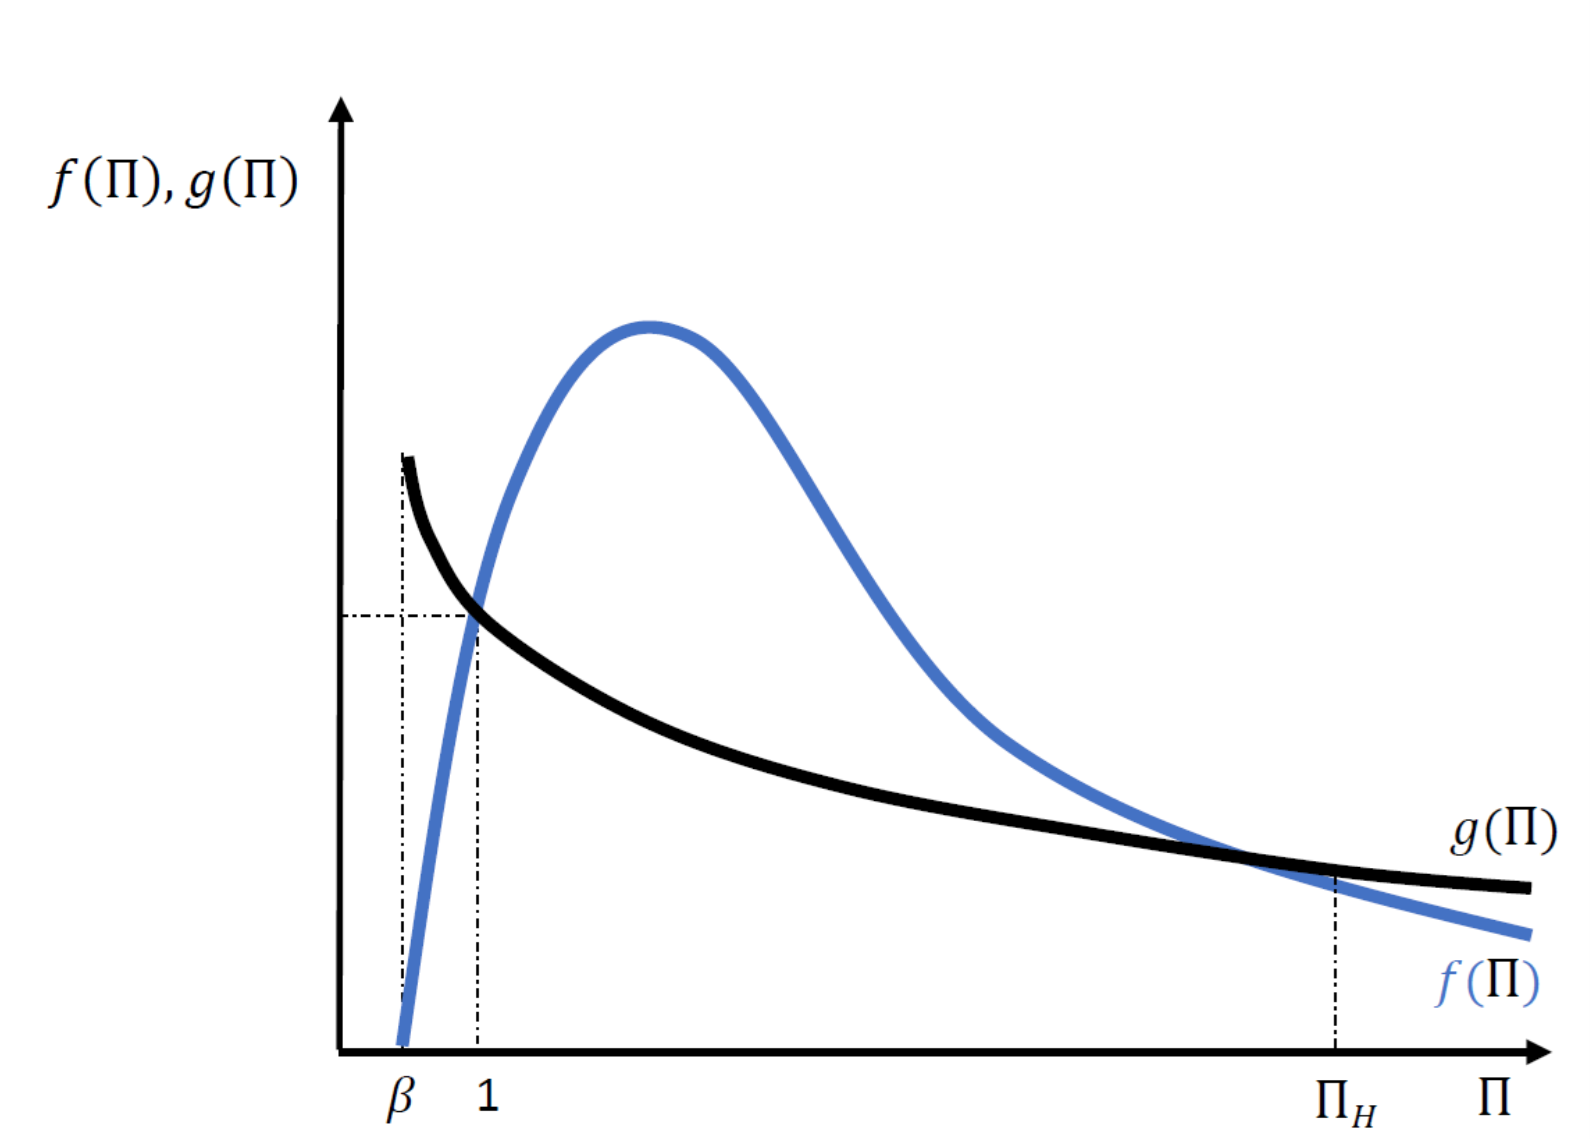
\includegraphics[width=0.6\linewidth]{Figures/Figure30.PNG}
    \par
\vspace{0.2cm}
    \textit{\tiny Solutions of Eq. (\ref{Eq.Central BankCentral Bank}) with $n_{t_{0}-1}^{C}=-1$: $g(\Pi )$ requirement vs. $f(\Pi )$ seigniorage.}
\end{figure}
\end{frame}

% -----------------------------------------------------------
\begin{frame}{Insolvency and the Limits of Independence}
\small
Negative net worth can trigger hyperinflationary dynamics even when the central bank is formally independent of the Treasury:

\begin{itemize}
    \item \textbf{Backing requirement:} To sustain the value of money, the central bank needs real backing. Without Treasury support, backing can only come from the value of its own assets.
    \item \textbf{Asset defaults:} If the central bank’s assets suffer large losses (e.g., widespread defaults), net worth can become sufficiently negative to create an immediate inflation risk.
    \item \textbf{Policy interaction:} Depending on the interest-rate rule, balance-sheet losses can generate accelerating inflation and, in extreme cases, hyperinflation.
    \item \textbf{Portfolio importance:} The composition and risk of the asset portfolio matter for inflation control—even under full institutional separation from the Treasury.
\end{itemize}
\end{frame}

% -----------------------------------------------------------
\begin{frame}{Mitigation: The Role of Gold}
\small
Strategic management of the central bank’s portfolio can mitigate insolvency and prevent an inflationary outcome:

\begin{itemize}
    \item \textbf{Alternative revenue:} Holding and selling gold can generate revenues that offset losses on nominal assets.
    \item \textbf{Impact on solvency:} In this framework, such revenues reduce the magnitude of negative net worth (i.e., raise \(n_{t_{0}-1}^{C}\)).
    \item \textbf{Stability buffer:} By filling the balance-sheet \enquote{hole} at critical dates, real assets can prevent the need for an inflationary jump.
    \item \textbf{Conclusion:} Preserving the nominal anchor requires a sound balance sheet; asset-side resilience is as important as institutional independence.
\end{itemize}
\end{frame}

% ===================== SECTION: CONCLUSION =====================

\section{Main Takeaways}
\begin{frame}{Main Takeaways}
\small
\begin{itemize}
  \item \textbf{Fiat Phenomena}: Hyperinflations are inherently fiat-money phenomena; inconvertibility enables the unconstrained expansion of nominal liabilities.
  \item Strong empirical co-movement between money growth and inflation; real money demand collapses as rising inflation expectations increase the opportunity cost of holding cash.
  \item \textbf{Fiscal Dominance}: Explicit monetization subordinates monetary policy to the budget; seigniorage requirements for persistent deficits create feasibility constraints via a \textbf{Seigniorage Laffer Curve}.
  \item Under \textbf{implicit backing} (unpleasant arithmetic), fiscal capacity and outstanding liabilities constrain monetary policy even without direct monetization; ``tight money'' can shift inflation into the future (or require an inflation jump today).
  \item \textbf{Central Bank Solvency}: Formal independence is insufficient if the Central Bank has negative net worth; balance-sheet weakness can force inflationary seigniorage when fiscal remittances are bounded at zero.
\end{itemize}
\end{frame}

%===========================================================
\section{Bibliography}
%===========================================================

\begin{frame}[allowframebreaks]{References}
\printbibliography
\end{frame}

\end{document}
